\documentclass[journal,oneside,a4paper,onecolumn]{IEEEtran}

% Some very useful LaTeX packages include:
% (uncomment the ones you want to load)

% *** CITATION PACKAGES ***
%
\usepackage{cite}
% cite.sty was written by Donald Arseneau
% V1.6 and later of IEEEtran pre-defines the format of the cite.sty package
% \cite{} output to follow that of IEEE. Loading the cite package will
% result in citation numbers being automatically sorted and properly
% "compressed/ranged". e.g., [1], [9], [2], [7], [5], [6] without using
% cite.sty will become [1], [2], [5]--[7], [9] using cite.sty. cite.sty's
% \cite will automatically add leading space, if needed. Use cite.sty's
% noadjust option (cite.sty V3.8 and later) if you want to turn this off.
% cite.sty is already installed on most LaTeX systems. Be sure and use
% version 4.0 (2003-05-27) and later if using hyperref.sty. cite.sty does
% not currently provide for hyperlinked citations.
% The latest version can be obtained at:
% http://www.ctan.org/tex-archive/macros/latex/contrib/cite/
% The documentation is contained in the cite.sty file itself.


% *** GRAPHICS RELATED PACKAGES **
%
  \usepackage{graphicx}
  \graphicspath{{../Figures/}}
  \DeclareGraphicsExtensions{.pdf,.png}
  \usepackage{color}

% *** MATH PACKAGES ***
%
\usepackage[cmex10]{amsmath}
% A popular package from the American Mathematical Society that provides
% many useful and powerful commands for dealing with mathematics. If using
% it, be sure to load this package with the cmex10 option to ensure that
% only type 1 fonts will utilized at all point sizes. Without this option,
% it is possible that some math symbols, particularly those within
% footnotes, will be rendered in bitmap form which will result in a
% document that can not be IEEE Xplore compliant!
%
% Also, note that the amsmath package sets \interdisplaylinepenalty to 10000
% thus preventing page breaks from occurring within multiline equations. Use:
%\interdisplaylinepenalty=2500
% after loading amsmath to restore such page breaks as IEEEtran.cls normally
% does. amsmath.sty is already installed on most LaTeX systems. The latest
% version and documentation can be obtained at:
% http://www.ctan.org/tex-archive/macros/latex/required/amslatex/math/

%\usepackage{amssymb}%............................ AMS Symbol fonts



% *** SPECIALIZED LIST PACKAGES ***
%
%\usepackage{algorithmic}
% algorithmic.sty was written by Peter Williams and Rogerio Brito.
% This package provides an algorithmic environment for describing algorithms.
% You can use the algorithmic environment in-text or within a figure
% environment to provide for a floating algorithm. Do NOT use the algorithm
% floating environment provided by algorithm.sty (by the same authors) or
% algorithm2e.sty (by Christophe Fiorio) as IEEE does not use dedicated
% algorithm float types and packages that provide these will not provide
% correct IEEE style captions. The latest version and documentation of
% algorithmic.sty can be obtained at:
% http://www.ctan.org/tex-archive/macros/latex/contrib/algorithms/
% There is also a support site at:
% http://algorithms.berlios.de/index.html
% Also of interest may be the (relatively newer and more customizable)
% algorithmicx.sty package by Szasz Janos:
% http://www.ctan.org/tex-archive/macros/latex/contrib/algorithmicx/

% *** ALIGNMENT PACKAGES ***
%
\usepackage{array}
% Frank Mittelbach's and David Carlisle's array.sty patches and improves
% the standard LaTeX2e array and tabular environments to provide better
% appearance and additional user controls. As the default LaTeX2e table
% generation code is lacking to the point of almost being broken with
% respect to the quality of the end results, all users are strongly
% advised to use an enhanced (at the very least that provided by array.sty)
% set of table tools. array.sty is already installed on most systems. The
% latest version and documentation can be obtained at:
% http://www.ctan.org/tex-archive/macros/latex/required/tools/


\usepackage{mdwmath}
\usepackage{mdwtab}
% Also highly recommended is Mark Wooding's extremely powerful MDW tools,
% especially mdwmath.sty and mdwtab.sty which are used to format equations
% and tables, respectively. The MDWtools set is already installed on most
% LaTeX systems. The lastest version and documentation is available at:
% http://www.ctan.org/tex-archive/macros/latex/contrib/mdwtools/

% IEEEtran contains the IEEEeqnarray family of commands that can be used to
% generate multiline equations as well as matrices, tables, etc., of high
% quality.

% *** SUBFIGURE PACKAGES ***
% subfig.sty, also written by Steven Douglas Cochran, is the modern
% replacement for subfigure.sty. However, subfig.sty requires and
% automatically loads Axel Sommerfeldt's caption.sty which will override
% IEEEtran.cls handling of captions and this will result in nonIEEE style
% figure/table captions. To prevent this problem, be sure and preload
% caption.sty with its "caption=false" package option. This is will preserve
% IEEEtran.cls handing of captions. Version 1.3 (2005/06/28) and later
% (recommended due to many improvements over 1.2) of subfig.sty supports
% the caption=false option directly:
\usepackage[caption=false,font=footnotesize]{subfig}
%
% The latest version and documentation can be obtained at:
% http://www.ctan.org/tex-archive/macros/latex/contrib/subfig/
% The latest version and documentation of caption.sty can be obtained at:
% http://www.ctan.org/tex-archive/macros/latex/contrib/caption/

%Setting captions to centered (Not IEEE journal standard)
\makeatletter
\long\def\@makecaption#1#2{\ifx\@captype\@IEEEtablestring%
\footnotesize\begin{center}{\normalfont\footnotesize #1}\\
{\normalfont\footnotesize\scshape #2}\end{center}%
\@IEEEtablecaptionsepspace
\else
\@IEEEfigurecaptionsepspace
\setbox\@tempboxa\hbox{\normalfont\footnotesize {#1.}~~ #2}%
\ifdim \wd\@tempboxa >\hsize%
\setbox\@tempboxa\hbox{\normalfont\footnotesize {#1.}~~ }%
\parbox[t]{\hsize}{\normalfont\footnotesize \noindent\unhbox\@tempboxa#2}%
\else
\hbox to\hsize{\normalfont\footnotesize\hfil\box\@tempboxa\hfil}\fi\fi}
\makeatother


% *** FLOAT PACKAGES ***
%
\usepackage{fixltx2e}
% fixltx2e, the successor to the earlier fix2col.sty, was written by
% Frank Mittelbach and David Carlisle. This package corrects a few problems
% in the LaTeX2e kernel, the most notable of which is that in current
% LaTeX2e releases, the ordering of single and double column floats is not
% guaranteed to be preserved. Thus, an unpatched LaTeX2e can allow a
% single column figure to be placed prior to an earlier double column
% figure. The latest version and documentation can be found at:
% http://www.ctan.org/tex-archive/macros/latex/base/

% *** PDF, URL AND HYPERLINK PACKAGES ***
%
\usepackage{url}

\usepackage{sistyle}
    \SIstyle{S-Africa}
    \SIunitspace{{\cdot}}
    \SIunitdot{{\cdot}}

% generate nice bookmarks and hyperrefs when exporting to pdf and dvi (screen version):
\usepackage[a4paper,plainpages=false,colorlinks,linktocpage,bookmarks=true,bookmarksopen=false]{hyperref}
% use this for printing only (no color, print version):
%\usepackage[a4paper,plainpages=false,colorlinks=false,linktocpage,bookmarks=true,bookmarksopen=false]{hyperref}

% correct bad hyphenation here
\hyphenation{op-tical net-works semi-conduc-tor}

%List of acronyms used in text
 \usepackage{acronym}%.......................... Acronym package to handle acronyms in text

\usepackage{floatflt}% This is used to flow text around some figures.

\acrodef{MMOG}{Massively Multiplayer Online Game}
\acrodef{MMORPG}{Massively Multiplayer Online Role Playing Game}
\acrodef{WoW}{World of Warcraft}
\acrodef{MUD}{Multi-User Dungeon}
\acrodef{PvP}{Player-versus-Player}
\acrodef{P2P}{Peer-to-Peer}
\acrodef{CS}[C/S]{Client/Server}
\acrodef{CMS}[C/MS]{Client/Multi-Server}
\acrodef{NPC}{Non-Player Character}
\acrodef{aoi}[AoI]{Area of Interest}
\acrodef{alm}[ALM]{Application Level Multicast}
\acrodef{ui}[UI]{User Interface}
\acrodef{DHT}{Distributed Hash Table}

\begin{document}

%
% paper title
\title{Request for Player Trace Data}

\author{\IEEEauthorblockN{John S. Gilmore\\}
\IEEEauthorblockA{MIH Media Lab\\
Department of Electronic Engineering\\
Stellenbosch University\\
Stellenbosch, South Africa\\
Email: jgilmore@ml.sun.ac.za}}

% make the title area
\maketitle

\hfill September, 2010

\section{Introduction}


\IEEEPARstart{T}{his} document describes what data is requested from Astrium, concerning the game ``Allods Online''. It presents a brief project
background, followed by a discussion of the data required as well as suggestions on some limitations that might be placed on the data, in order to
ease server load during the collection process. The documents concludes by asking some questions on how Allods stores data at the server.

\section{Background}

We are currently doing research into Peer-to-Peer (P2P) Massively Multiplayer Online Games (MMOGs). One challenge that is present in this field is
how to move from a centralised storage database at the server, to a fully distributed database, hosted over all peers. Another challenge is where to
host mutable game objects, such as doors that can be open or closed, or vodka bottles that can be full, empty or half.

Methods have been found to address both of the mentioned issues, but we believe that we can improve upon these methods. Three methods for object
hosting exist: overlay-based, region-based and distance-based. In a region-based system, a single peer is promoted to super peer status and acts as a
server for a specific region. The super peer hosts all objects and maintains object persistency. Hand-over mechanisms are used to promote another
peer to super peer status, after the current super peer for a region has left.

The second method used is distance-based storage. Distance-based storage hosts all objects on the computer of the player, closest to the object being
hosted. This creates a significant amount of handover overhead, but has the advantage that object access times for players near objects are very low.

Overlay storage equally distributes game objects over all peer in the network, by making use of a distributed hash table. In this scheme, objects are
evenly spread out, which means that the load is also evenly spread. The problem with this hosting scheme is that it incurs high latencies, because of
the P2P overlay being created, which incurs a routing cost of $O(\log(n))$.

Each of these methods to distribute and store objects have their own advantages and disadvantages. We are, however, looking at a completely new
object hosting paradigm that would more naturally distribute game objects and allow for a two-tiered hybrid approach to game state persistency. This
new paradigm is that of using player groups to distribute objects over. Player objects can then be shared amongst groups of players, instead of a
single player, with added quorum (voting) mechanisms implemented in the group to ensure the integrity of the P2P system.

We believe that building an MMOG based on groups will allow us to solve many issues related to, not only P2P MMOGs, but also Client/Server MMOGs. For
the grouping paradigm to be successful, the hypothesis that players usually move in groups and interact with other players in groups should first be
established.

\section{Trace data requirements}

With this grouping paradigm in mind, there are a few areas that we would like to investigate:
\begin{enumerate}
\item How players move around in the virtual world.
\item Player density in different game areas.
\item Grouping behaviour of players, if any.
\item Whether player groups may be programmatically extracted.
\item Average group sizes.
\item Group movement speed.
\item Group churn. (How many players leave and join a group.)
\end{enumerate}

To be able to observe this behaviour, player trace data for specific types of in-game areas are required. What is required from all data traces are:
that all players in the data set be uniquely identified and that it be possible to observe player movements over time. No detailed player information
is currently required. Some player identifier is sufficient for the traces as the level and motivation for player movements will not currently be
explored.

The issue has been raised about how the amount of data collected could be decreased, so not as to introduce lag into the server. Two proposed methods
were to only select a random sub-set of the total number of players and another was to only record player positions every set number of trace steps.
Other methods that might also be used to reduce server load is to only monitor players in a limited geographic area and only monitor them for as long
as is required. It's difficult to give a clear cut answer to any of these questions, as one would prefer to have as detailed player data as possible.

A discussion of how the amount of data may be reduced follows, but what should be kept in mind is that these reductions are completely subject to
what is possible on the server side. We would also like the option to continue the data collection process and to submit more data requests after the
first request's data has been processed. It is believed that this should be an iterative process, with further data requests to follow after a
previous data set has been processed. The reason for this is, for example, exploring different level zones and experimenting with more or less trace
steps.

\subsection{Geographic limitation}

\begin{floatingfigure}[l]{0.5\textwidth}
\centering
 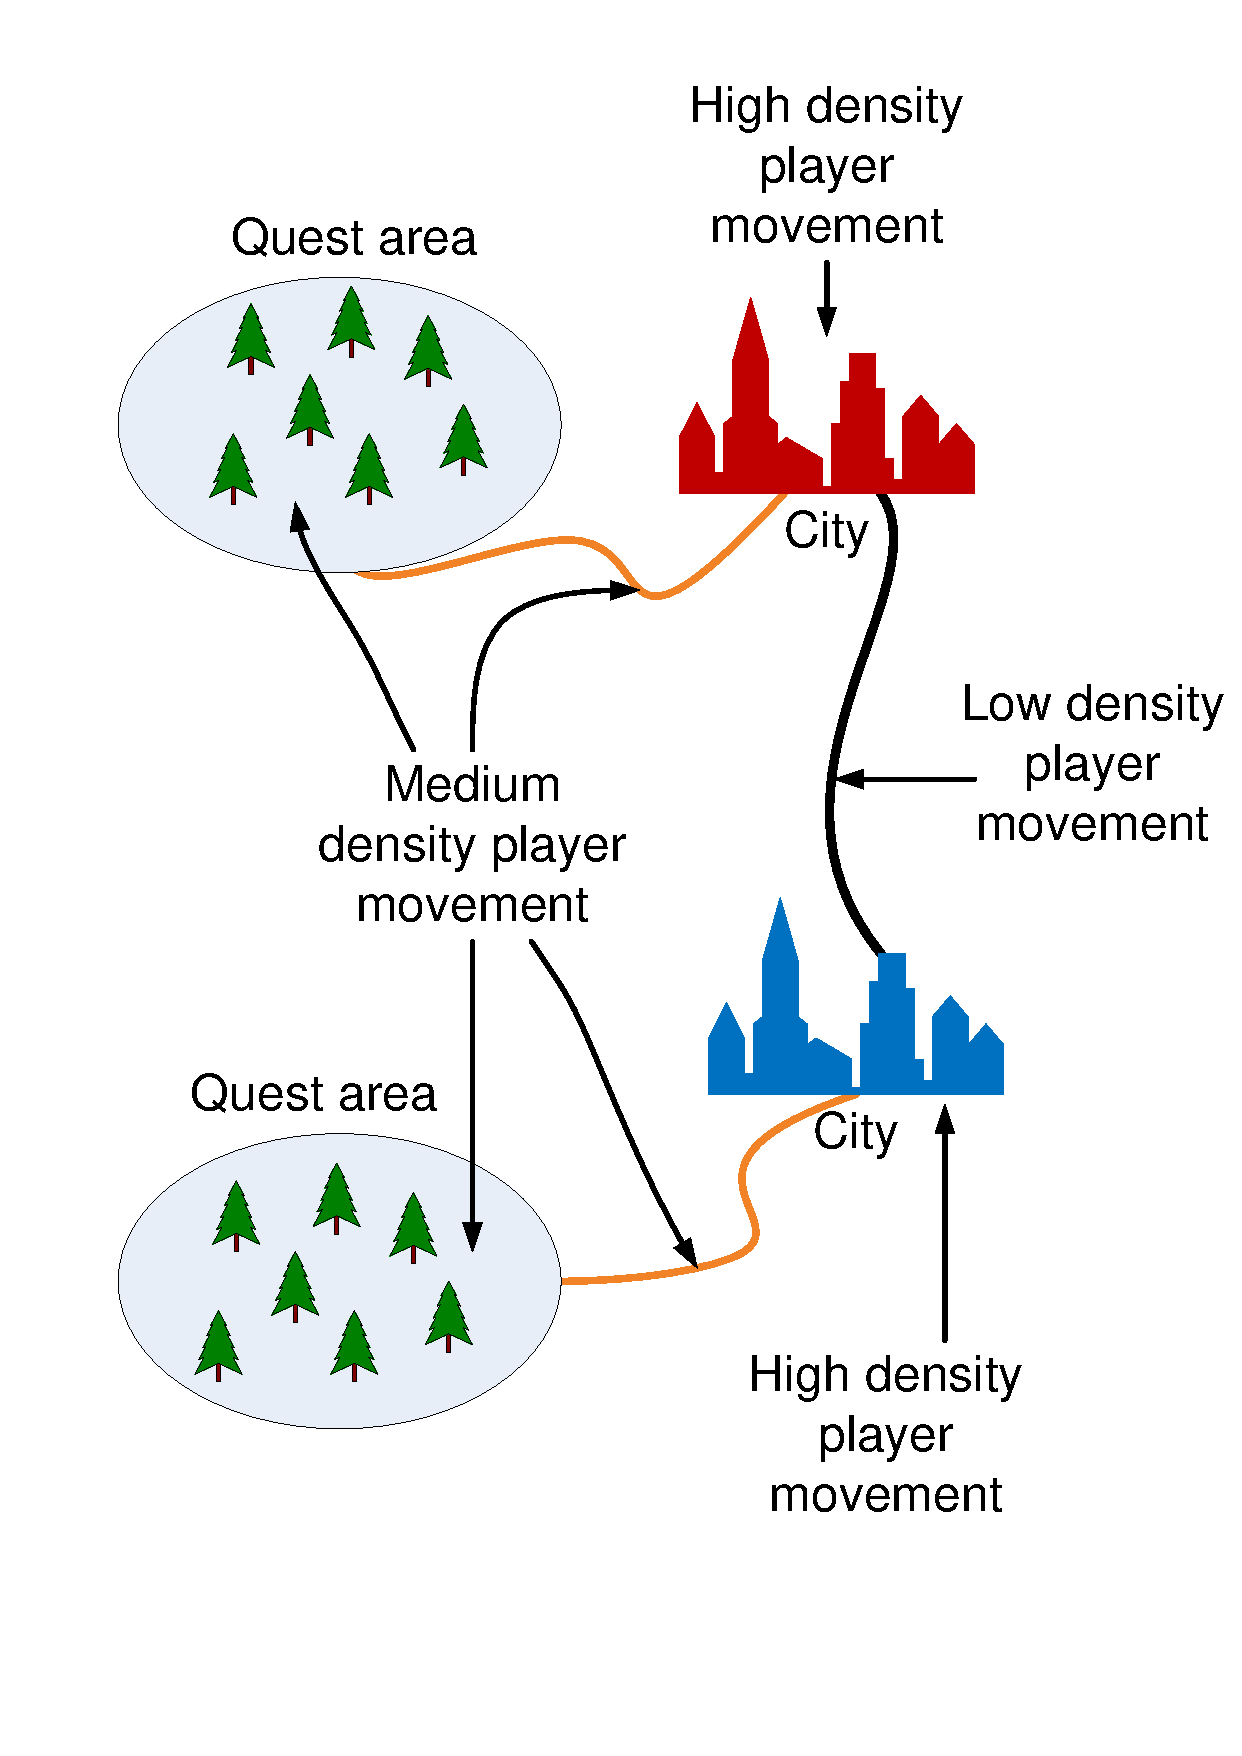
\includegraphics[width=0.5\textwidth]{Player_density_expectations}
 \caption{This figure shows the expected player density of players in a virtual world.}
 \label{fig_player_density}
\end{floatingfigure}
%
If we first look at limiting the geographic area, there are a few areas of interest where player behaviour might be different. This first area is
that of an NPC questing area, where players receive quests in a city, perform these quests outside the city and then return to the city to complete
quests and trade with NPC traders. The expected player density of this area is shown in Figure \ref{fig_player_density}. It is expected that a very
high player density will be present in the city, with many players moving around, mostly on their own, to complete quests and trade.

Outside the city, there are usually areas where quests can be done. These quests are usually in the form of kill $x$ number of NPC and return to the
quest giver once this number of NPCs have been killed. These NPCs can usually be found in a very specific region near to where the quest was given.
There are usually many quests to be done and many (sometimes overlapping) areas in which to complete these quests. We would like to monitor player
movements in such a ``questing'' region. We would also like to monitor player movement in low and high level areas, to determine the difference in
player behaviour in these areas. It is expected that higher level areas will show more player grouping, since teamwork is required to complete these
areas. Some movement is also expected in areas between cities, by players travelling from one level area into another, higher or lower level, area.

Other areas that are also of interest are Player versus Player (PvP) areas. Here, a strong element of grouping is also expected, with one or more
groups in direct opposition to each other. The movement of one group in these areas is expected to be very dependant on the movement of the
opposition group.

The areas that are currently of interest are:
\begin{enumerate}
\item A low level area around a town or city, that contains some areas where quests are completed.
\item A high level area around a town of city, that contains some areas where high level quests are completed.
\item Inside a large city.
\item A PvP area, where groups of players usually clash.
\end{enumerate}
%
All areas should contain a sufficient number of players to be able to perceive a grouping behaviour, if one is present. All areas should also be
sufficiently large to contain one or more groups of players, if these groups are present.

\subsection{Player limitation}

It should be possible to randomly select a limited number of players, out of the complete set of players, and still obtain usable data. What is
important is that grouping behaviour should still be detectable after player elimination. The sizes of the groups that can be detected will depend on
the ratio of player elimination. For example, if one out of five players is randomly selected to be traced, groups of five and smaller players will
not be detectable.

The choice of elimination ratio then depends on the average group size of players in the game and also on which areas are traced. For cities, it is
estimated that selecting one out of every twenty players in the city will be sufficient. For the areas outside the low level cities, one out of every
three players would be more appropriate as small group sizes are expected. This should not be such a problem, since the total population is also much
lower in these areas. In higher level areas, one out of every five or ten players might be sufficient.

It is important to point out that these are merely guidelines, since what is possible on the server is not known. As many players as possible should
be monitored and the number of monitored players should be chosen as a total number of players for every zone. What is meant by this is that if there
exits one zone with 10 players in, and another with 50 players, one should rather choose to always monitor a maximum of 20 players, rather than a
ratio of players. Monitoring one in five players will monitor 2 players in the first zone and ten in the seconds. If ten players van be monitored,
all ten might just as well be monitored in the first scenario.

\subsection{Trace step limitation}

One should play around with the trace step, to determine what time works best. After running around a bit in Allods, it seems that three or five
seconds should be sufficient for now. Again, one would have to take a look at the trace data to try and determine what works best. What would
probably be done in the future is doing a trade-off between trace step time and number of players monitored.

Again, these times are also merely guidelines and what is possible should be determined by the developers.

\section{Database access information}

On a different topic from game traces, we also have some questions about the database access requirements of Allods Online. Part of my PhD is
designing a low latency distributed storage medium, specifically tailored to MMOGs. This storage medium will be where the P2P architecture stores all
data. Currently there are distributed storage mediums available, but these mediums have lengthy access times. Some examples are PAST, OceanStore and
Freenet.

These file storage systems have been specifically developed for file storage and retrieval, and secrecy, but not for online games. These systems act
more as file archives, with no real-time availability. What we would like to know is whether there is space for such a distributed storage with
real-time access capabilities? Also, we would like to know what the types of data are that are stored in the server database, how regularly the data
are stored and retrieved, and how much of each type of data flows into and out of the database over a certain period of time.

These types of classifications will assist in our distributed file storage architecture and assist us in tailoring the architecture specifically to
online games.

\section{Conclusion}

In this data request, a brief project history was provided. The reason for the data request was discussed and reductions that might be made to the
data were given. These were: limiting the areas, limiting the player numbers, and limiting the trace steps used.

It is understood that the required data will be a few different data sets, that contain the data of different areas. It should be noted that the
required data does not have to be given as one large set, but that data sets can be sent to us, as soon as the data for the scenario has been
collected. This will allow for data mining to commence as soon as some data are ready to be worked on. The other sets may be sent through as is
convenient for your developers.

Some more information was also requested on what, when and how much data Allods stores and retrieves to and from the database. Answering these
questions will assist in the development of the distributed game state persistency mechanism that we're working on.

% that's all folks
\end{document}
